\section{Mission Overview}

\subsection{Mission Definition}
The Cluster-II Mission is planned and executed by the European Space Agency and was launched on 16th of July 2016. The whole mission consists of four identical spacecrafts flying in a tetrahedral formation in a highly elliptical orbit, where each spacecraft is collecting various data on the space environment with its 11 scientific payload instruments. These in-situ measurements are done to build a very accurate 3D-Model of the earth's magnetosphere and thus to observe the magnetosphere interaction with the solar wind not only in a spatial but also in a temporal resolution.

The main goal of this mission is to examine and gather data especially on the plasma structures in the bow shock region, the magnetopause, polar cusps, the earth's magnetotail and the auroral zone, all of them regions with very interesting properties when it comes to the interaction with solar wind \citep{ESA:clusterWebsite}.

\begin{figure}[h]
	\centering
	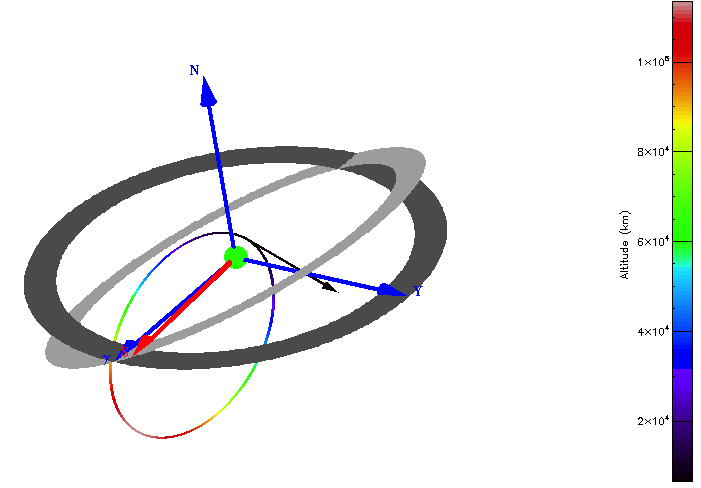
\includegraphics[width=\linewidth-15em]{spenvis/3d_gei}
		\caption{One Orbit of FM-8 Tango, the color bar shows the altitude}
	\label{fig:orbit}
\end{figure}
To model the Orbit of FM-8 Tango a set of TLE\footnote{Two Line Element} data provided by CelesTrak was used \citep{celesTrak}.\\
Figure \ref{fig:orbit} shows one orbit of FM-8 Tango and indicates the altitude of the orbit. The orbit itself is a retrograde orbit with an inclination of 131.6 degrees. A complete set of TLE data describing all important orbit parameters can be found in the Appendix \ref{tleParameters}.
\begin{figure}[H]
%	\centering
%	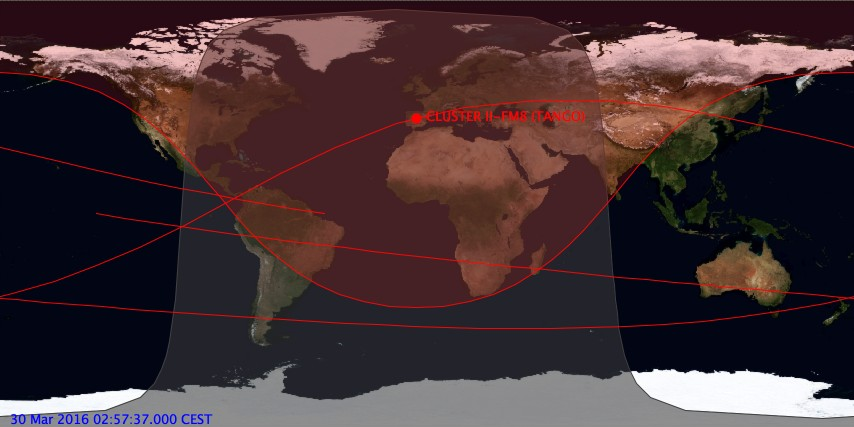
\includegraphics[width=\linewidth-5em]{spenvis/tango_groundtrack}
%		\caption{Groundtrack of one Tango Orbit, image provided by JSatTrack \citep{jsattrack}}
%	\label{fig:groundtrack}
%\end{figure}
%\begin{figure}[h]
	\centering
	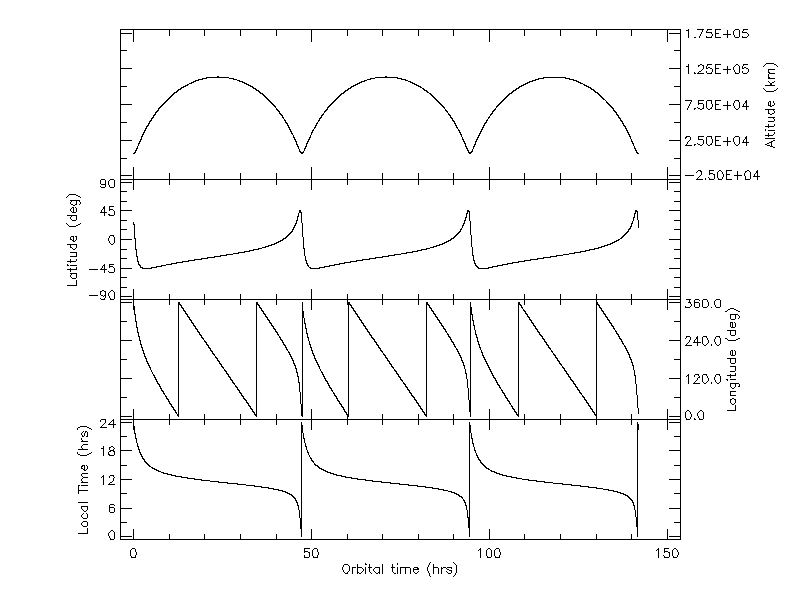
\includegraphics[width=\linewidth-15em]{spenvis/cans}
		\caption{Various Data on 3 orbits of FM8 Tango}
	\label{fig:orbitData}
\end{figure}


\subsection{Space Environment}

\begin{figure}[h]
	\centering
	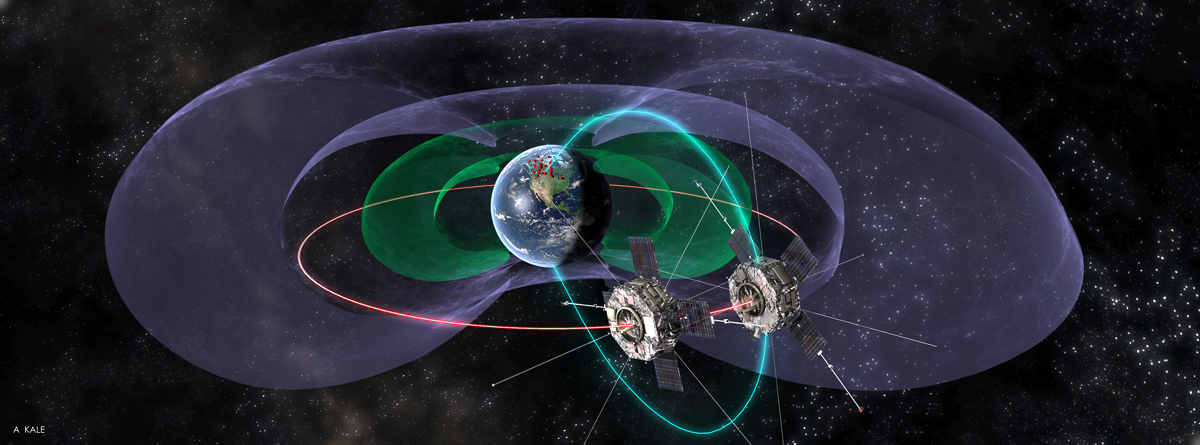
\includegraphics[width=\linewidth+5em]{images/mysteriesofe}
		\caption{Van Allen Probes in the Van Allen Belt by \href{http://cdn.phys.org/newman/gfx/news/hires/2013/mysteriesofe.jpg}{phys.org}}
	\label{fig:worldmap}
\end{figure}

Due to its highly elliptical orbit as seen in Fig.\ref{fig:orbit} and the relatively high perigee of 28000km and apogee of 104000km the satellite moves through different space environments, as for example the Van Allen Belt, and encounters different particles and plasma configurations on its way, which may lead to Spacecraft Charging and other effects, but may also be affected by Micrometeoroids and Space Debris, the so-called MMOD environment. Since these environments may be hazardous for the satellite, a proper investigation and analysis of these effects is necessary to ensure a proper satellite operation during its lifetime.

\begin{figure}[H]
	\centering
	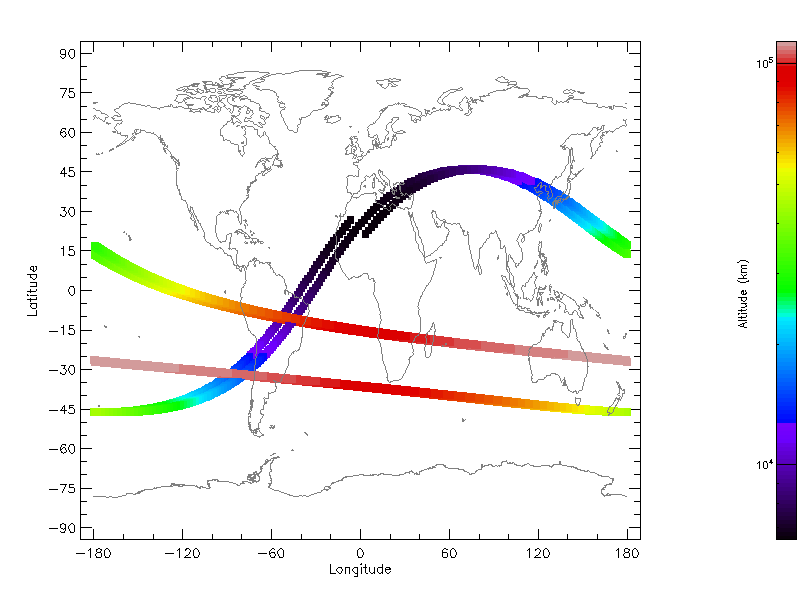
\includegraphics[width=\linewidth-15em]{spenvis/worldmap_2_orb}
		\caption{Groundtrack of 2 FM8 Tango Orbits}
	\label{fig:worldmap}
\end{figure}

\begin{figure}[H]
	\centering
	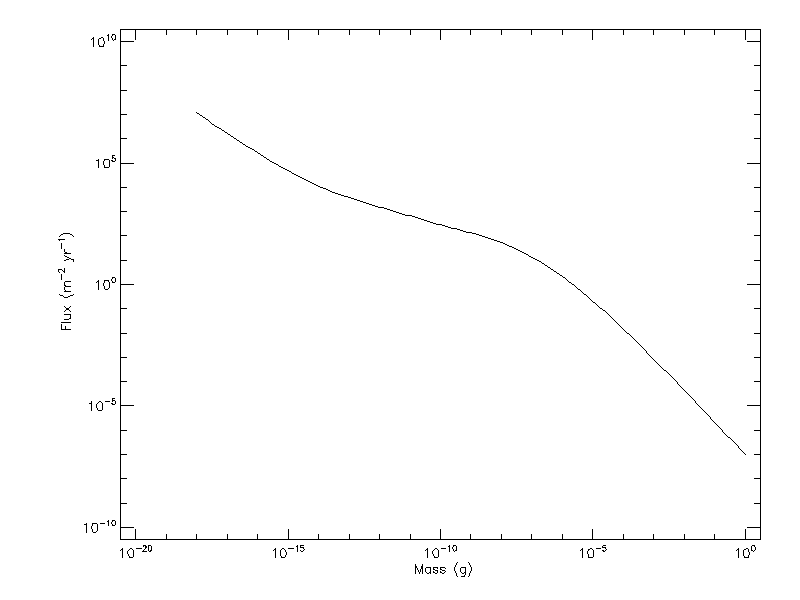
\includegraphics[width=\linewidth-15em]{spenvis/meteoroid_perigee}
		\caption{Flux of Meteoroids compared to their mass at perigee}
	\label{fig:perigee_mmod}
\end{figure}


An important point is the MMOD environment. Usually micrometeoroids and space debris also play a important role in the space environment a satellite encounters. Although in our case this is only a minor factor, since we expect most micrometeoroids and space debris to be in lower orbits. This is backed by our findings with the help of SPENVIS as may be seen in Figure \ref{fig:perigee_mmod}.



\subsection{Drag and Atmospheric Oxygen}
But not only the MMOD environment exposes the spacecraft to risks. It is the atmosphere of the earth that affects the satellite in terms of drag forces, which occur due to the bombardment with atmospheric particles and slow the spacecraft down. Another risk is the Atomic Oxygen, which itself is highly reactive and degrades the spacecraft outer surfaces.

Since our chosen mission is in a quite high orbit, atmospheric effects do not play a big role and can be neglected \citep{vallado2008}. Our simulations with SPENVIS support this statement, as can be seen in Figures \ref{fig:atmox}. Only during the perigee the satellite encounters some particles, which are in the magnitude of $10^{-20}$ to $10^{-30}$ and thus can be neglected.

%\begin{figure}[h]
%	\centering
%	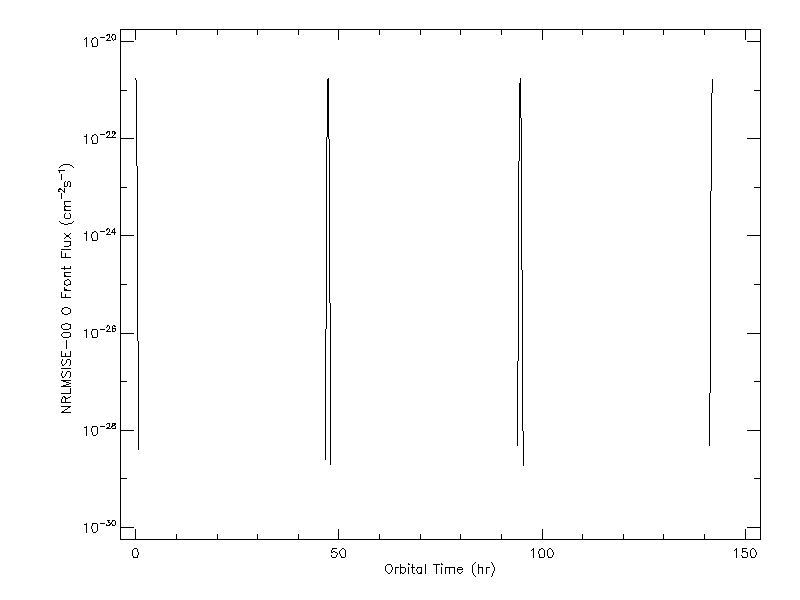
\includegraphics[width=\linewidth-15em]{spenvis/atomox_time}
%		\caption{Front Flux of Oxygen during 3 Orbits}
%	\label{fig:atmox}
%\end{figure}
%
%\begin{figure}[h]
%	\centering
%	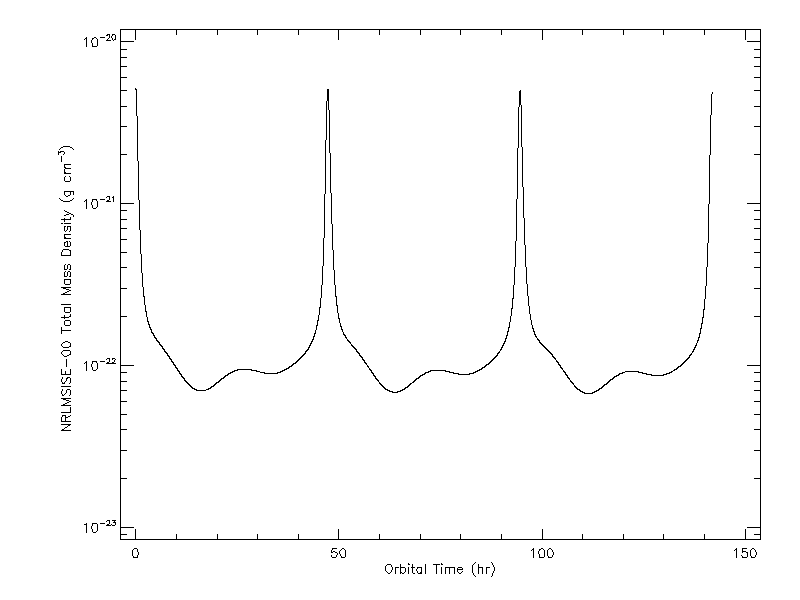
\includegraphics[width=\linewidth-15em]{spenvis/atomox_total_mass_density}
%		\caption{Total Mass Density during 3 Orbits}
%	\label{fig:atmox_drag}
%\end{figure}

\begin{figure}[!htbp]
  \centering
  \begin{minipage}[b]{0.45\textwidth}
	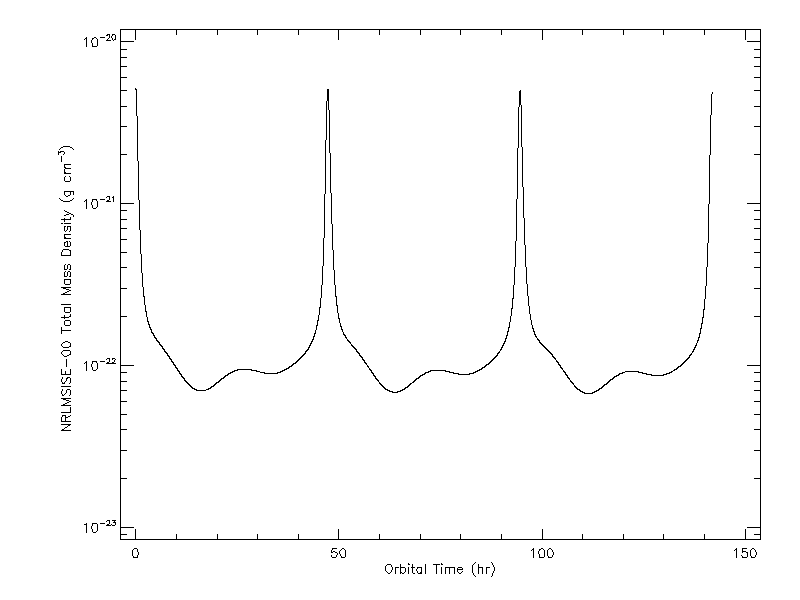
\includegraphics[width=\textwidth]{spenvis/atomox_total_mass_density}
		\caption{Total Mass Density during 3 Orbits}
	\label{fig:atmox_drag}
  \end{minipage}
  \hfill
  \begin{minipage}[b]{0.45\textwidth}
	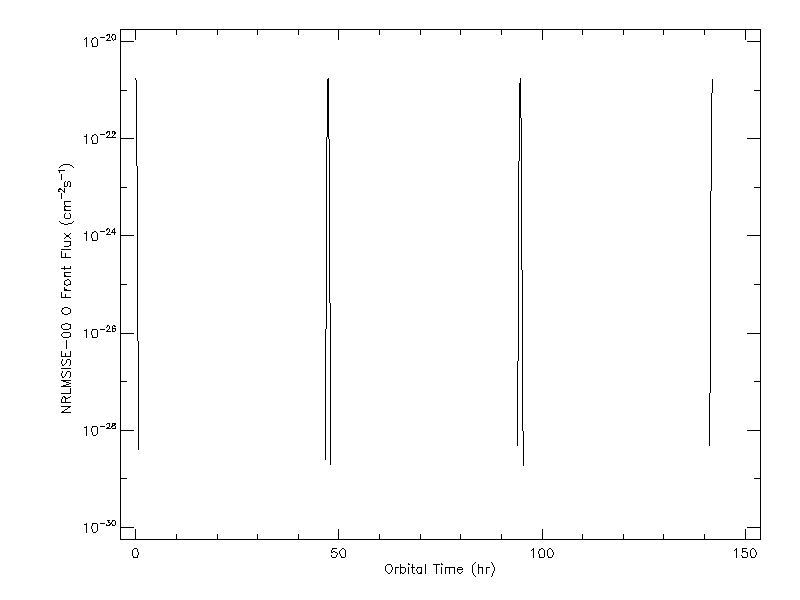
\includegraphics[width=\textwidth]{spenvis/atomox_time}
		\caption{Front Flux of Oxygen during 3 Orbits}
	\label{fig:atmox}

  \end{minipage}
\end{figure}




\subsection{Plasma Environment}
\begin{figure}[!htbp]
  \centering
  \begin{minipage}[b]{0.45\textwidth}
    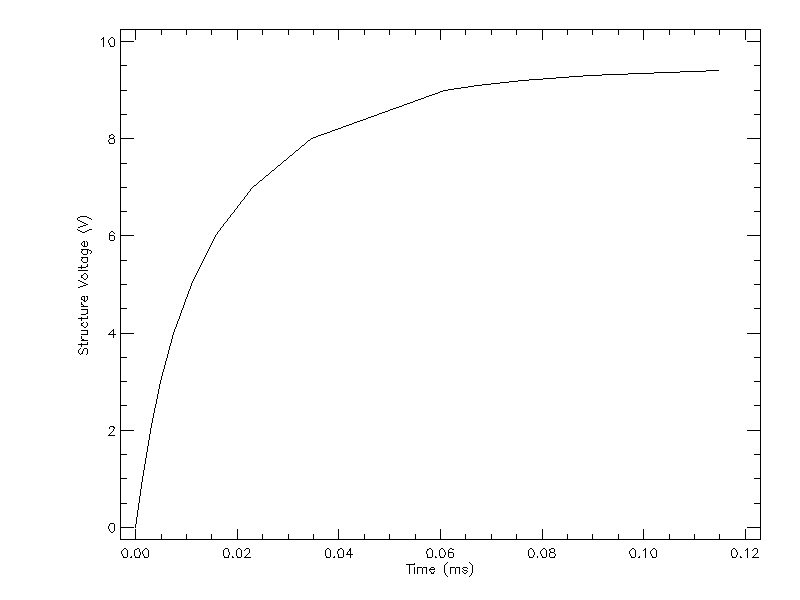
\includegraphics[width=\textwidth]{spenvis/sunlight_voltage}
    \caption{Structure Voltage in Sunlight}
    \label{fig:volt_sun}
  \end{minipage}
  \hfill
  \begin{minipage}[b]{0.45\textwidth}
    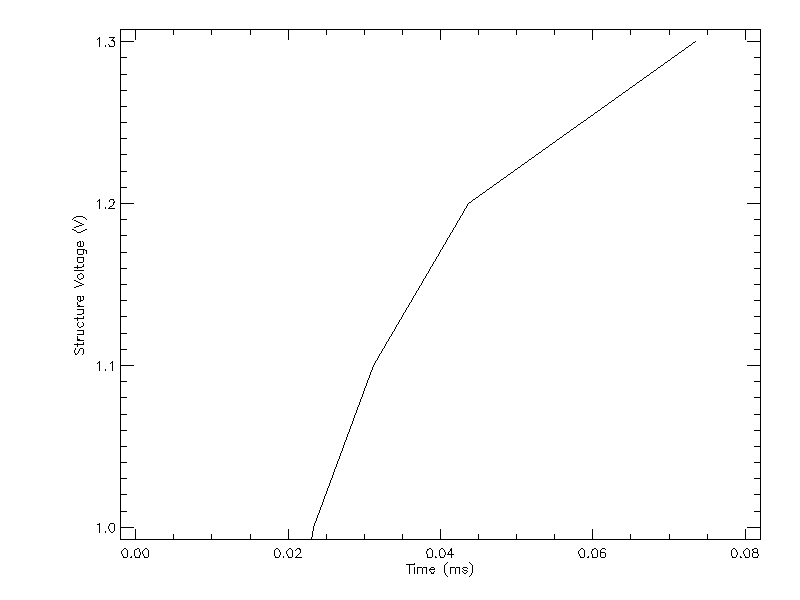
\includegraphics[width=\textwidth]{spenvis/eclipse_voltage}
    \caption{Structure Voltage in Eclipse}
    \label{fig:volt_eclipse}
  \end{minipage}
\end{figure}

As already stated and is well known, the Van Allen belts extend from about 100km to 65000km and consists of two so-called "belts", whereas newer findings suggest a belt in-between them as well \citep{ecss:10-04C}. Since the FM-8 satellite's lowest point is its perigee, it only moves through the outer Van Allen Belt, where the satellite is bombarded with ions and electrons. 
Due to this bombardment the satellite gains a potential compared to its surrounding plasma, called the floating potential. The floating potential depends on multiple parameters, some of them being the flux of ions and electrons hitting the surface area of the satellite and photoionisation, when in sunlight.
Usually spacecrafts in higher orbits gain a negative structure potential, since the electrons have a smaller mass and thus are faster and more energetic in terms of their thermal energy.

%Due to the higher thermal energy of the electrons, since they are smaller and faster than the ions, the Spacecraft accumulates a high negative potential,
Running simulations on the satellite's potential we had some interesting findings, since the satellite's structure Voltage is positive. This is due to the fact, that FM-8 is almost always in the sunlight, it is bombarded with high-energy Ions, which leads to a positive structure potential, as may be seen in Fig. \ref{fig:volt_sun}. And since FM-8 is only about seven minutes in eclipse during one orbit, the Potential stays positive during this time as well.




A detailed analysis on the necessary shielding will be explained in detail in Chapter \ref{chap:dose}.


